\documentclass{article}
\usepackage[utf8]{inputenc}
\usepackage[a4paper, total={6in,10in}]{geometry}
\usepackage{amsmath}
\usepackage{bm}
\usepackage{amssymb}
\usepackage{graphicx}
\title{Hand-in assignments \\ PhD course on Sequential Monte Carlo methods 2019}
\author{\textbf{Martin Hellkvist}\\
	 \textit{Signals and Systems, Uppsala University}}

\begin{document}
\maketitle
\subsection*{H.1 Importance sampling theory}
\paragraph{(a)} Show that the estimator $\hat{Z}$ is unbiased.

\textbf{Solution:} Plug the estimator $\hat{Z}=\frac{1}{N}\sum_{i=1}^N \frac{\tilde{\pi}(x^i)}{q(x^i)}$ into the expectation:
\begin{align}
	\mathbb{E}[\hat{Z}] = \frac{1}{N}\sum_{i=1}^{N}\mathbb{E}\frac{\tilde{\pi}(x^i)}{q(x^i)} = \frac{1}{N}N\mathbb{E}_X\frac{\tilde{\pi}(x)}{q(x)}, 
\end{align}
where the last equality holds because the expectation is constant w.r.t the samples $x^i$. Using the definition of expectation, and that $\tilde{\pi}(x):= Z\pi(x)$ the expression becomes:
\begin{align}
	\mathbb{E}[\hat{Z}]= \int \frac{\tilde{\pi}(x)}{q(x)}q(x)dx = \int \tilde{\pi}(x)dx = \int Z \pi(x) dx= Z\int\pi(x)dx = Z.
\end{align}
So the expectation of the estimate is exactly the true value, hence the estimator is unbiased.

\paragraph{(b)}
Using the Cauchy distribution as proposal, implement an IS that samples from the standard normal distribution. Find the gamma that minimizes the asymptotic variance of the IS and provide plots for the approximation of the normalizing constant $\sqrt{2\pi}$.

\textbf{Solution:} the function to minimize is $ \int\pi^2(x)/q(x)dx -1 $:
\begin{equation}
\gamma^* = \arg\min_{\gamma>0} \int\frac{\pi^2(x)}{q(x)}dx -1 = \arg\min_{\gamma>0} \int\frac{\pi^2(x)}{q(x)}dx = \arg\min_{\gamma>0} f(\gamma).
\end{equation}
Plugging in the expressions $\pi(x) = \frac{1}{\sqrt{2\pi}}\exp\{-x^2/2\}$ and $q(x)=\frac{\gamma}{\pi(\gamma^2+x^2)}$, the function $f(\gamma)$ becomes
	\begin{equation}
		f(\gamma) = \int\frac{\pi^2(x)}{q(x)}dx = \int \frac{1}{2\pi}\frac{\exp\{-x^2\}}{\frac{\gamma}{\pi(\gamma^2+x^2)}}dx = \int \frac{\exp\{-x^2\}}{2}\frac{\gamma^2+x^2}{\gamma} dx =
	\end{equation}
	\begin{equation}
		= \int \frac{\gamma^2}{2\gamma}\exp\{-x^2\}dx + \int \frac{1}{2\gamma}x^2\exp\{-x^2\}dx.
	\end{equation}
The integration is over the whole real axis for $x$, and the expression becomes
	\begin{equation}
		f(\gamma)=\dfrac{\gamma^2}{4\gamma}\sqrt(\pi)\text{erf}(x) + \dfrac{1}{8\gamma}\Big(\sqrt(\pi)\text{erf}(x)-2\exp\{-x^2\}x\Big)\Bigg|_{x\rightarrow-\infty}^{x\rightarrow+\infty}=
	\end{equation}
	\begin{equation}
		=\dfrac{(2\gamma^2+1)\sqrt{\pi}\text{erf}(x)-2\exp\{-x^2\}x}{8\gamma}\Bigg|_{x\rightarrow-\infty}^{x\rightarrow+\infty} =
	\end{equation}
	\begin{equation}
		= \dfrac{\Big((2\gamma^2+1)\sqrt{\pi}\cdot 1 - 2\cdot 0\Big) - \Big((2\gamma^2+1)\sqrt{\pi}\cdot(-1) - 2\cdot 0\Big)}{8\gamma} = \dfrac{(2\gamma^2 +1 )}{4\gamma}\sqrt{\pi},
	\end{equation}
where $\text{erf}(x):= \dfrac{2}{\sqrt{\pi}}\int_{0}^{x}e^{-t^2}dt$ is the \textit{error function}.

The function $f(\gamma)/\sqrt{\pi} = \frac{(2\gamma^2+1)}{4\gamma }= \frac{\gamma}{2} + \frac{1}{4\gamma}$ is convex for $\gamma>0$ and has a unique minimum at $\gamma^*\rightarrow \frac{d}{d\gamma} \Big(\frac{\gamma}{2}+\frac{1}{4\gamma}\Big) =0$ which is found as
	\begin{equation}
		\dfrac{1}{2} - \dfrac{1}{4\gamma^2} = 0 \Leftrightarrow \gamma = 1/\sqrt{2}.
	\end{equation}
\begin{figure}
	\centering
	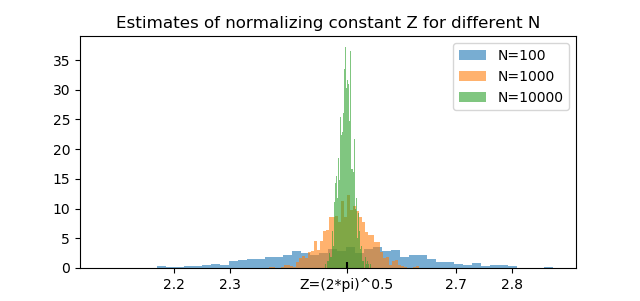
\includegraphics[width=0.7\linewidth]{1_b_hist_newg}
	\caption{For three different values of $N$ we see different variance in the estimate of Z. As $N$ increases, the variance decreases. The average of each histogram is close to the true value $Z=\sqrt{2\pi}$. The histogram was generated with 1000 simulations for each N.} 
	\label{fig:1bhist}
\end{figure}
The simulation results illustrated in figure \ref{fig:1bhist} demonstrates how the implemented IS is unbiased.

\paragraph{(c)} Now target the Cauchy distribution using the standard normal distribution.

\textbf{Solution: } The variance of the estimator is now
	\begin{equation}
		\int \dfrac{\pi^2(x)}{q(x)}dx - 1  = \int \dfrac{\gamma^2}{\pi^2(\gamma^2+x^2)^2}\dfrac{1}{\frac{1}{\sqrt{2\pi}}\exp\{-x^2/2\}}dx -1=\int \dfrac{\gamma^2}{\pi^2(\gamma^2+x^2)^2}\sqrt{2\pi}\exp\{x^2\}dx-1,
	\end{equation}
	which does not converge, i.e., the variance is infinite. Although the estimator is theoretically unbiased, it is numerically infeasible to attain an unbiased estimate.
	
%A problem arises here which is that the proposal explores a too small range of the target.
%The narrow exploration generates too many large weights, making the distribution of the estimate skewed.
%When $N$ increases, the estimated average approaches the true value $\pi$.
%
%If we increase the variance of the proposal from 1 to 20, giving it heavier tails the implementation clearly illustrates the unbiasedness even for $ N=100 $.
%%
Figure \ref{fig:1chist1} illustrates the IS with the standard normal distribution as proposal, and figure \ref{fig:1chist2} instead shows the histograms generated with the normal distribution with standard deviation 20 instead. An increased variance of the proposal decreases the bias that is actually implicitly introduced by this infinite variance.

\begin{figure}[h]
	\centering
	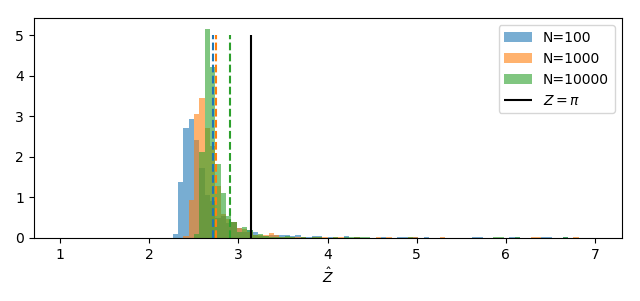
\includegraphics[width=.7\linewidth]{1_c_hist1}
	\caption{Task 1c. The distribution of the estimated normalization was skewed due to thin tails of the proposal.}
	\label{fig:1chist1}
\end{figure}
\begin{figure}[h]
	\centering
	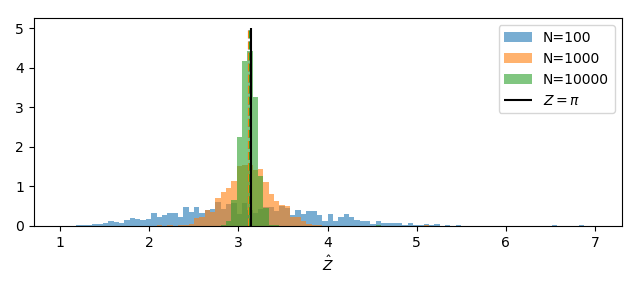
\includegraphics[width=.7\linewidth]{1_c_hist2}
	\caption{Task 1c. When the tails of the proposal were heavier, the estimates clearly clearly illustrated the unbiasedness of the IS.}
	\label{fig:1chist2}
\end{figure}





\subsection*{H.2 Particle filter for a linear Gaussian state}
\paragraph{(a)} The pdf's are $p(x_t|x_{t-1}) = \mathcal{N}(x_t; 0.8x_{t-1}, 0.5)$ and $ p(y_t|x_t) = \mathcal{N}(y_t;2x_t, 0.1) $.

\paragraph{(b)} Because we perfectly know the noise covariances, and that the model matches the simulated system, the Kalman filter is the optimal linear filter. The particle filter is on the other hand can model nonlinearities is the data. Therefore, we can expect the particle filter's estimated trajectory to be closer to the true one, if we number of particles is large enough.

\paragraph{(c)} After implementing the bootstrap filter, the variance was computed for each $N$ as $Var(\hat{x}_t) = \sum_{i=1}^{N}w_t^i (x_t^i)^2 + \big(\sum_{i=1}^{N} w_t^i x_t^i \big)^2$. The Kalman filter's variance converges after only a few iterations. The variances are plotted in figure \ref{fig:2_c}.

Letting MAD denote the absolute difference between the BPF state estimate and the Kalman state estimate, averaged over time, the results together with average variance of the BPF is presented in table \ref{tab:2c}.
\begin{table}
	\centering
	\begin{tabular}{lrr}\hline
		$N$ & MAD 		& Variance 	\\
		10 	& 0.1489	& 0.020  	\\
		50	& 0.0412	& 0.023		\\
		100	& 0.0271	& 0.023		\\
		2000& 0.0060	& 0.024		\\
		5000& 0.0042 	& 0.024		\\
		Kalman & 0.0000 & 0.025		\\\hline
	\end{tabular}
	\caption{2c. Simulation results for the Bootstrap Particle filter}
	\label{tab:2c}
\end{table}

\begin{figure}[h]
	\centering
	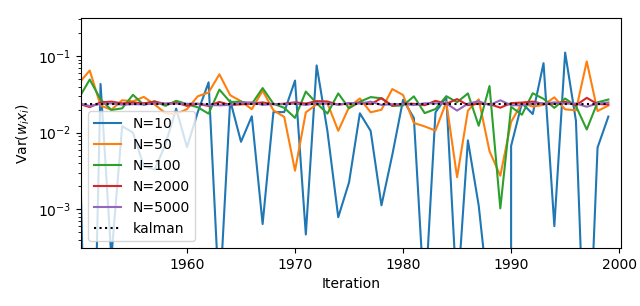
\includegraphics[width=.7\linewidth]{2_c}
	\caption{2c. Variance over particles per iteration of the BPF state estimates compared to the Kalman variance.}
	\label{fig:2_c}
\end{figure}

\paragraph{(d)} Derivation of the Fully Adapted Particle Filter pdf's follows.
The first proposal, for the adjustment multipliers $\bm{\nu}$:
	\begin{equation}
		\nu_{t-1}^i = p(y_t|x_{t-1}^i) = \dfrac{p(y_t,x_{t-1}^i)}{p(x_{t-1}^i)} \propto p(y_t,x_{t-1}^i).
	\end{equation}
	From the probabilistic model we have 
	\begin{equation}
		\mathcal{N}(y_t; 2x_t^i,0.1),
	\end{equation}
	from which we can plug in the model for $x_t^i$:
	\begin{equation}
		\mathcal{N}(y_t; 2(0.8x_{t-1}^i+V_t),0.1) = \mathcal{N}(y_t; 1.6x_{t-1}^i + 2V_t,0.1) = \mathcal{N}(y_t; 1.6x_{t-1}^i,4\cdot 0.5 + 0.1),
	\end{equation}
	thus, we have 
	\begin{equation}
		p(y_t|x_{t-1}^i) = \mathcal{N}(y_t; 1.6x_{t-1}^i, 2.1).
	\end{equation}
	
For the optimal proposal $q$:
	\begin{align}
		q(x_t|x_{t-1}, y_t) &\propto p(y_t|x_t,x_{t-1})p(x_t|x_{t-1}) = \mathcal{N}(y_t;2x_t,0.1)\mathcal{N}(x_t; 0.8x_{t.1},0.5) \propto\\
		&\propto \exp\{-\dfrac{(y_t-2x_t)^2}{2\cdot 0.1}\}\exp\{-\dfrac{(x_t-0.8x_{t-1})^2}{2\cdot 0.5}\}\propto\\
		&\propto\exp\{-\dfrac{(x_t-\frac{1}{42}(20y_t-1.6x_{t-1}))^2}{2\frac{1}{42}}\},
	\end{align}
so we get the normal distribution q:
	\begin{equation}
		q(x_t|x_{t-1}, y_t) = \mathcal{N}(x_t;~\frac{1}{42}(20y_t-1.6x_{t-1}), \frac{1}{42})
	\end{equation}


Table \ref{tab:2d} presents the MAD between the FAPF and the Kalman state trajectories for one simulation. Compared to the results for the BPF, the MAD is now a lot lower for small N, while they are still lower for larger N's but not as strikingly. 
\begin{table}
	\centering
	\begin{tabular}{lrr}\hline
		$N$ & MAD 		\\
		10 	& 0.0388	\\
		50	& 0.0181	\\
		100	& 0.0122	\\
		2000& 0.0028	\\
		5000& 0.0019 	\\\hline
	\end{tabular}
	\caption{2d. The mean average difference between the Fully Adapted Particle filter's state trajectory and the Kalman filter's state trajectory.}
	\label{tab:2d}
\end{table}

\paragraph{(e)} Figure \ref{fig:2_e} illustrates how only a few particles at time 1950 are remaining as ancestors for the final particles. 

\begin{figure}[h]
	\centering
	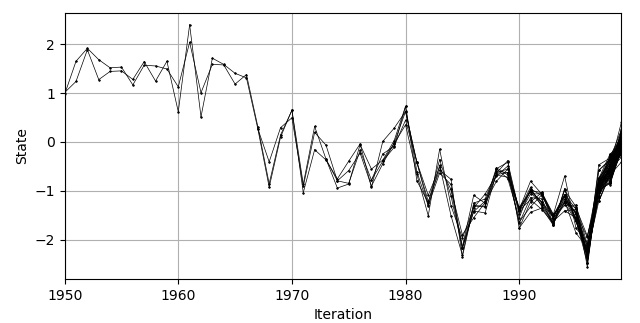
\includegraphics[width=\linewidth]{2_e}
	\caption{2e. Particle genealogy from time 1950 to 1999 for the fully adaptive particle filter.}
	\label{fig:2_e}
\end{figure}

\paragraph{(f)} With systematic resampling the FAPF obtains less degeneracy and the final particles have many more ancestors. As illustrated in figure \ref{fig:2_f}, at iteration 2 there are around 30 particles who are ancestors to the final 100 particles.
\begin{figure}[h]
	\centering
	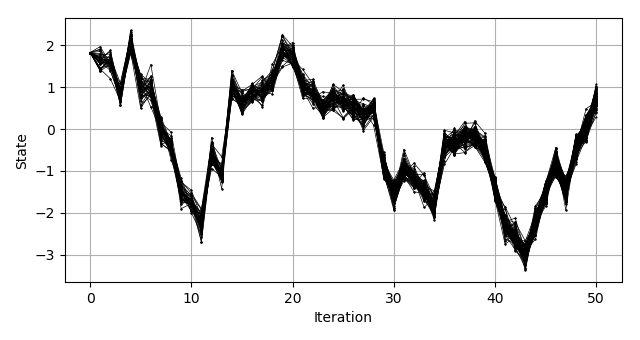
\includegraphics[width=\linewidth]{2_f}
	\caption{2f. The early genealogy for the final 100 particles.}
	\label{fig:2_f}
\end{figure}
\end{document}	